\documentclass[tikz,border=8pt]{standalone}
% Shared look for every TikZ diagram. Load with \input{../../tools/tikz-style.tex}
\usepackage[T1]{fontenc}
\usepackage{lmodern}
\renewcommand{\sfdefault}{lmr}  % diagrams use the same serif as the text
\usetikzlibrary{arrows.meta, positioning, shapes.geometric, calc, fit, backgrounds}
\definecolor{cblue}{HTML}{4C78A8}
\definecolor{corange}{HTML}{F58518}
\definecolor{cgreen}{HTML}{54A24B}
\definecolor{cred}{HTML}{E45756}
\definecolor{cpurple}{HTML}{B279A2}
\definecolor{cgrey}{HTML}{6B6B6B}
\tikzset{
  every picture/.style={font=\sffamily, line width=1.2pt},
  box/.style={draw=#1, fill=#1!12, rounded corners=4pt, align=center, inner sep=7pt, minimum height=1.1cm},
  box/.default=cgrey,
  arrow/.style={-{Stealth[length=3mm]}, draw=cgrey, line width=1.4pt},
  title/.style={font=\sffamily\bfseries\Large},
  note/.style={font=\sffamily\small, text=cgrey, align=center},
}
\AtBeginDocument{\hyphenpenalty=10000 \exhyphenpenalty=10000}

\begin{document}
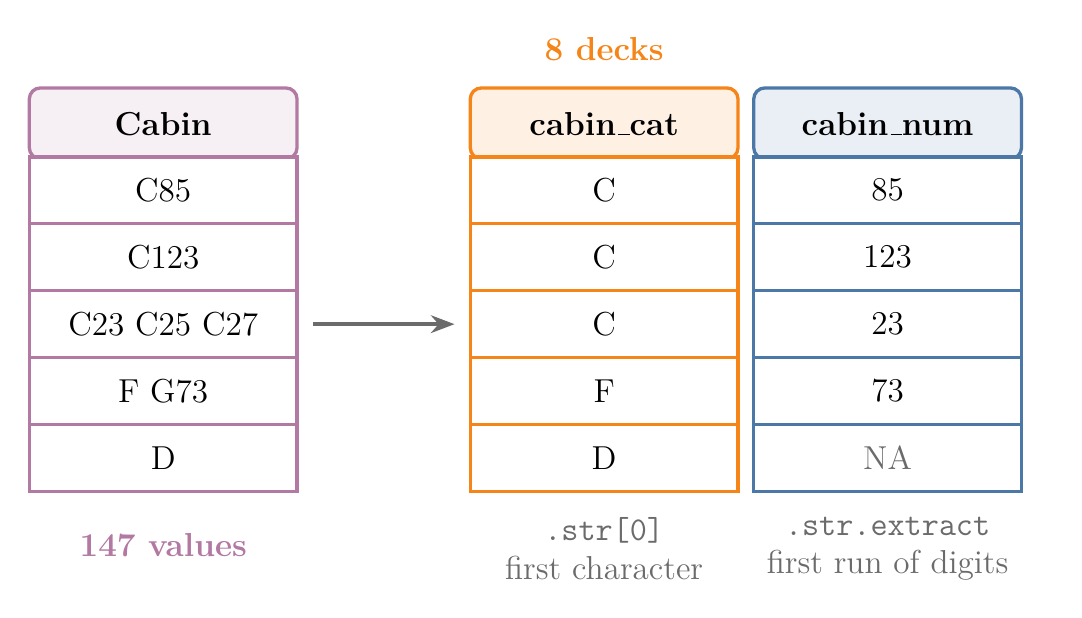
\begin{tikzpicture}[every node/.append style={font=\sffamily\large}]
\tikzset{note/.style={font=\sffamily\large, text=cgrey, align=center}}
  \tikzset{cl/.style={draw=#1, fill=white, minimum width=3.4cm, minimum height=0.85cm},
           hd/.style={box=#1, minimum width=3.4cm, minimum height=0.9cm, inner sep=3pt}}
  \node[hd=cpurple] at (0,0) {\textbf{Cabin}};
  \node[hd=corange] at (5.6,0) {\textbf{cabin\_cat}};
  \node[hd=cblue] at (9.2,0) {\textbf{cabin\_num}};
  \foreach \a/\b/\n [count=\i] in {C85/C/85, C123/C/123, C23 C25 C27/C/23, F G73/F/73, D/D/\textcolor{cgrey}{NA}} {
    \node[cl=cpurple] at (0,-0.85*\i) {\a};
    \node[cl=corange] at (5.6,-0.85*\i) {\b};
    \node[cl=cblue] at (9.2,-0.85*\i) {\n};
  }
  \draw[arrow] (1.9,-2.55) -- (3.7,-2.55);
  \node[note, text width=4cm] at (5.6,-5.4) {\texttt{.str[0]}\\first character};
  \node[note, text width=4cm] at (9.2,-5.4) {\texttt{.str.extract}\\first run of digits};
  \node[font=\sffamily\bfseries\large, text=cpurple] at (0,-5.35) {147 values};
  \node[font=\sffamily\bfseries\large, text=corange] at (5.6,0.95) {8 decks};
\end{tikzpicture}
\end{document}
